%! TEX program = pdflatex

\documentclass[oneside,solution]{tmpl}

\usepackage[utf8]{inputenc}
\usepackage[english,ukrainian]{babel}

\title{Домашня робота}
\author{Захаров Дмитро}
\studentID{МП-31}
\instructor{Ігнатович С.Ю.}
\date{\today}
\duedate{23:59 25 березня, 2024}
\assignno{4}
\semester{Весняний семестр 2024}
\mainproblem{Математичний Маятник}

\begin{document}

\maketitle

% \startsolution[print]

\problem{Математичний маятник.}

\textbf{Умова.} Рух маятника з урахуванням тертя можна описати системою
\begin{equation*}
    \begin{cases}
        \dot{x} = y \\
        \dot{y} = -\omega^2 \sin x - \kappa y
    \end{cases},
\end{equation*}
де $\kappa>0$ -- коефіцієнт тертя. Як ви думаєте, як зміниться фазовий портрет порівняно з випадком $\kappa=0$? Що буде при малих $\kappa$, а що -- при великих $\kappa$? Перевірте Ваші передбачення за допомогою програми. 

\textbf{Розв'язок.} Інтуїтивно з початкового рівняння -- доданок $-\kappa y$ буде ``тормозити'' значення $y$, що є нашою кутовою швидкістю, а отже маятник рано чи пізно перейде у стан стійкої рівноваги $x=0$. Це означає як мінімум, що замкненість системи зникає. Більш того, оскільки ми з будь-якої точки рано чи пізно перейдемо у початкову, то наша фазова траєкторія буде ``закручуватись'' до точки рівноваги.

Характер цього ``затухання'' можна описати з параметру $\kappa$. Якщо $\kappa$ маленьке, то траєкторії будуть дуже повільно відхилятися від тих, що були при $\kappa=0$ (навколо стану рівноваги -- приблизно еліпси). Але якщо $\kappa$ стає великим, то траєкторії одразу відхиляються з початкових замкнених і різко прямують до $(2\pi k,0), k \in \mathbb{Z}$ -- стійких точок рівноваги. 

\textbf{Програма.} Використовуємо ту саму програму, що і була наведена, з однією зміною: замість
\begin{lstlisting}[language=Python]
def f(x,y):
    return y, -omega**2*np.sin(x) 
\end{lstlisting}
будемо використовувати:
\begin{lstlisting}[language=Python]
def f(x,y):
    return y, -omega**2*np.sin(x) - k*y
\end{lstlisting}

Також цікаво дослідити залежність портретів від $\kappa$, тому ми додатково зафіксуємо набір значень $\kappa$, по яким будемо проходитись, і для кожного побудуємо свій портрет. Програма для цього:
\begin{lstlisting}[language=Python]
for k in [0.01, 0.1, 0.3, 0.6, 1.0, 1.5, 2.0, 3.0, 5.0]:
    def f(x,y):
        return y, -omega**2*np.sin(x) - k*y
    
    fig = plt.figure(figsize=(10,5))
    ax = fig.add_subplot()
    ax.grid()
    ax.set_aspect('equal')
    
    x = np.linspace(-2*np.pi,2*np.pi,50)  
    y = np.linspace(-3,3,50)  
    xx, yy = np.meshgrid(x,y)
    
    f1,f2 = f(xx,yy)	
    ax.streamplot(xx,yy,f1,f2,density=1.8)
    
    fig.savefig(f'phase_{k}.png')
\end{lstlisting}

\begin{figure}
\begin{tabular}{cc}
  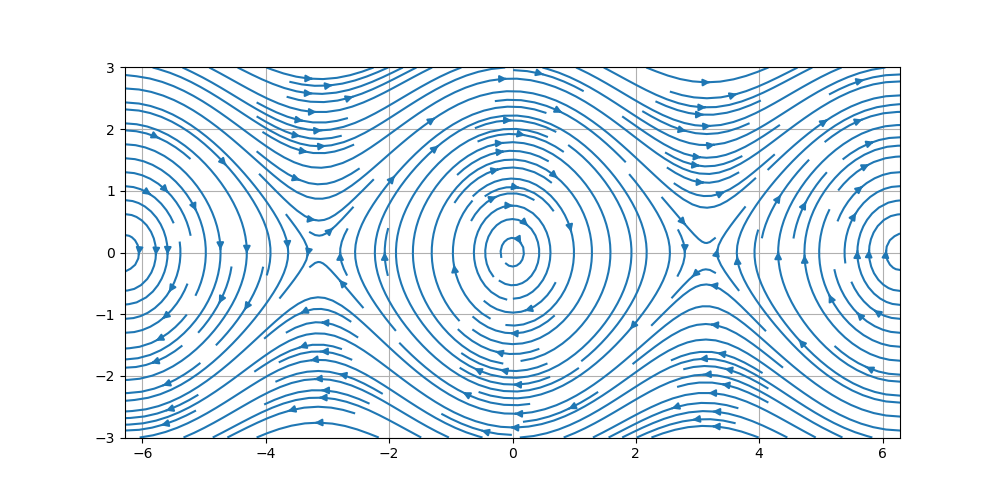
\includegraphics[width=0.5\textwidth]{images/hw_4/phase_0.01.png} &   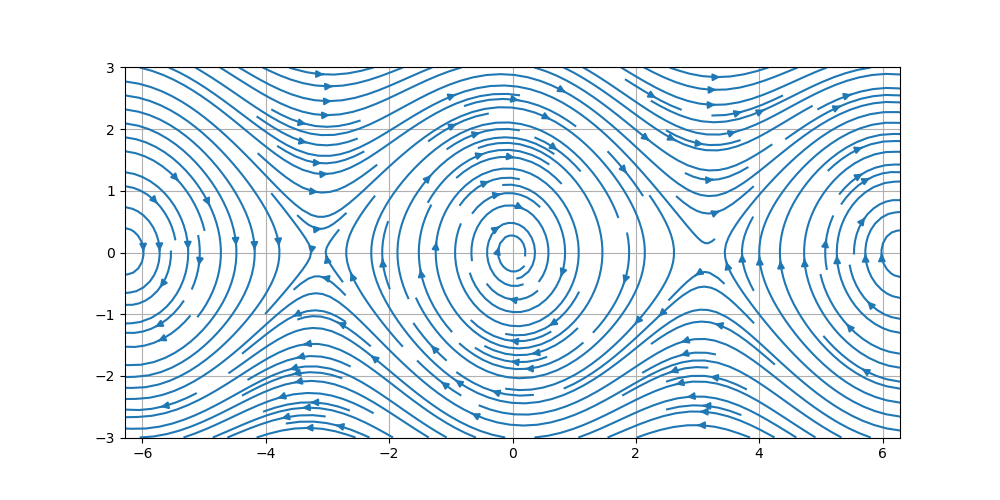
\includegraphics[width=0.5\textwidth]{images/hw_4/phase_0.1.png} \\
 $\kappa=0.01$ & $\kappa=0.1$ \\[6pt]
 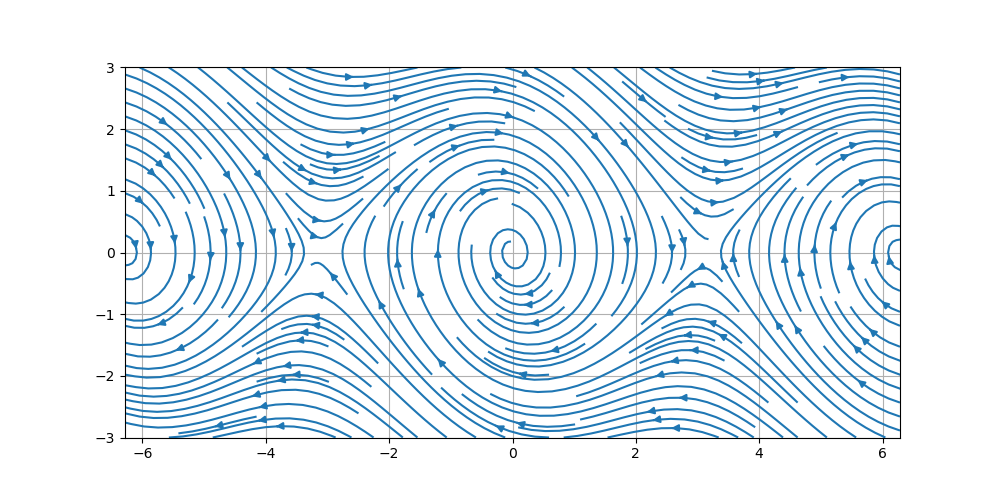
\includegraphics[width=0.5\textwidth]{images/hw_4/phase_0.3.png} &   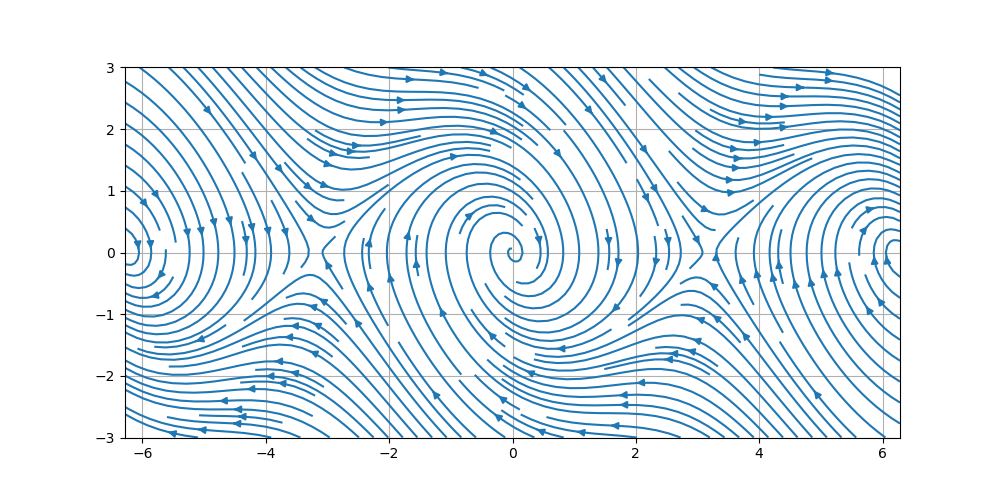
\includegraphics[width=0.5\textwidth]{images/hw_4/phase_0.6.png} \\
  $\kappa=0.3$ & $\kappa=0.6$ \\[6pt] \\[6pt]
 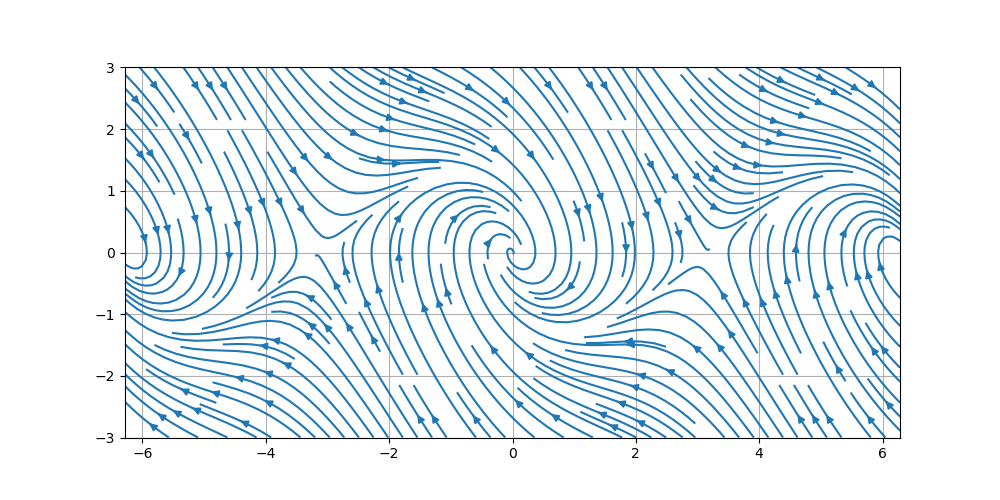
\includegraphics[width=0.5\textwidth]{images/hw_4/phase_1.0.png} &   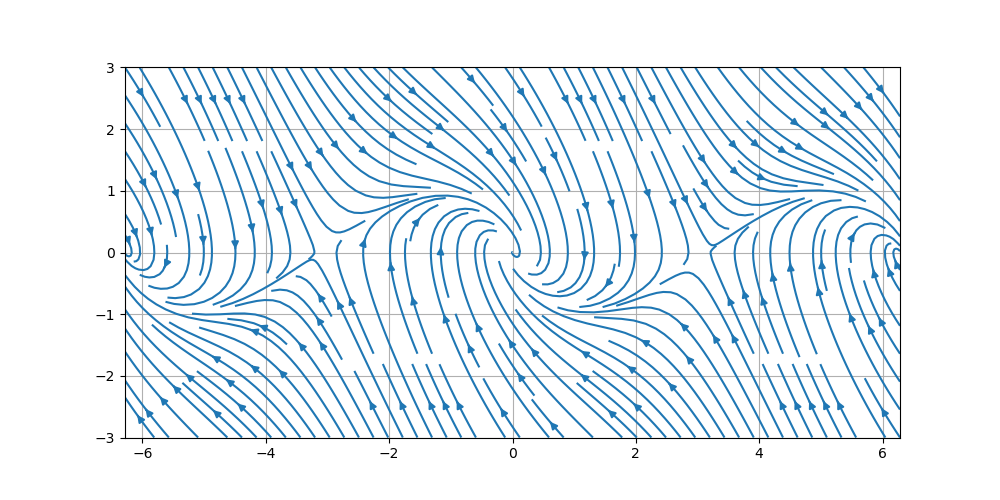
\includegraphics[width=0.5\textwidth]{images/hw_4/phase_1.5.png} \\
  $\kappa=1.0$ & $\kappa=1.5$ \\[6pt] \\[6pt]
 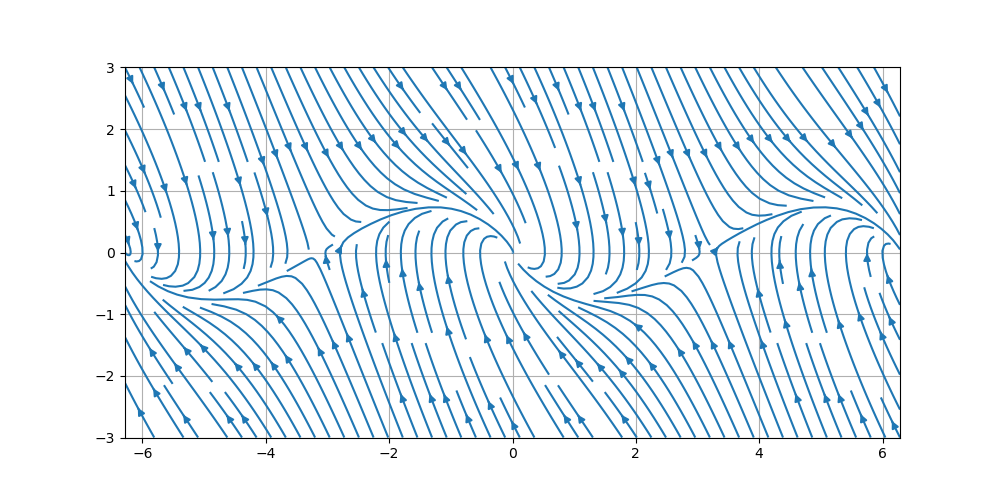
\includegraphics[width=0.5\textwidth]{images/hw_4/phase_2.0.png} &   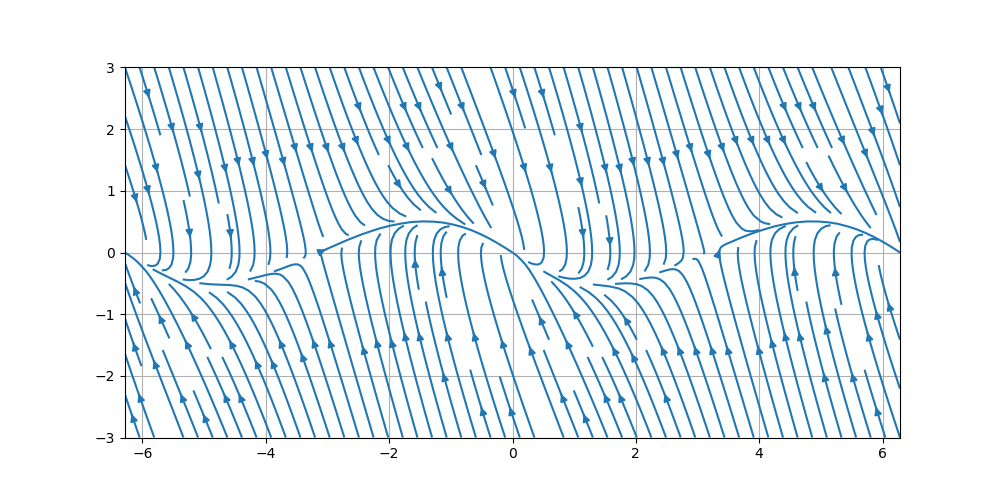
\includegraphics[width=0.5\textwidth]{images/hw_4/phase_3.0.png} \\
  $\kappa=2.0$ & $\kappa=3.0$ \\[6pt]
\end{tabular}
\caption{Фазові портрети при різних $\kappa$, кутову швидкість зафіксували $\omega=1.25$.}
\label{fig:phase}
\end{figure}

Результат зображено на рис. \ref{fig:phase}. Дійсно отримали те, що очікували: при малих $\kappa$ фазовий портрет майже не змінюється від випадку $\kappa=0$, а ось починаючи приблизно з $\kappa=0.6$ портрет стає цікавим: точка закручується навколо стійких точок рівноваги, постійно наближаючись до них. При зовсім великих $\kappa$, рух починає нагадувати рух по прямій.

\end{document}
